\documentclass{homework}
\author{Wiyninger, Caleb}
\class{CSCI 2114: Tashfeen's Data Structures}
\date{\today}
\title{Homework 3}
\address{%
  Oklahoma City University, %
  Petree College of Arts \& Sciences, %
  Computer Science%
}

\acmfonts

\newcommand\computerphile{\href{%
    https://www.youtube.com/watch?v=HXNhEYqFo0o%
  }{Programming Loops vs Recursion - Computerphile}}
\newcommand\download{\href{%
    https://tashfeen.org/s/ds/Experiment.java%
  }{Download}}

\begin{document} \maketitle

\question Point your favourite web-browser to \url{https:www.google.com}.
Perform a search for the term, ``recursion''. Why did you misspell
it? What happened?

\begin{sol}
I didnt, it recursively links to the same page 
\end{sol}

\question\label{vid} Watch the YouTube video \computerphile. Did you
learn something new? Can you think of something where you might opt
for recursion over loops?

\begin{sol}
  properly parsing nested code. Eg: A loop in a loop in a function in a class being called from another class. Depth first search. 
\end{sol}

\question Write a \texttt{public class Sorter} in Java that implements the
Java interface\footnote{Java interfaces are just abstract classes
  where all the interface methods are left to be implemented.
  Furthermore, a Java class may implement more than one interface
  but inherit from only one parent class.} given in listing
\ref{intr}. The sorter class may not have any methods other than
those which exist in the Godric's Hat interface.

% \lstinputlisting[
%   language={java},
%   caption={Java interface for different sorting algorithms.},
%   label=intr]
% {./code/GodricsHat.java}

The method \texttt{counting(int[] array)} is the same as
\texttt{sortIntegers(int[] toSort)} from the last homework. If you
wish, you may use the implementation from there.

While the following two methods,

\begin{verbatim}
void merge(int[] array);               // use recursion only
void quick(int[] array, int p, int r); // use recursion only
\end{verbatim}

must be implemented using recursion. The method,

\begin{verbatim}
void quickLoopy(int[] array);
\end{verbatim}

must be implemented iteratively \ie using only loops. The only
import statement you may have in the sorter class should import
the stack,

\begin{verbatim}
import java.util.Stack;
\end{verbatim}

The four algorithms you are implementing by implementing the
interface are,

\begin{enumerate}
  \item Insertion Sort
  \item Merge Sort
  \item Quick Sort (recursively)
  \item Quick Sort (loopy)
  \item Counting Sort (sometimes called a different name)
\end{enumerate}

Use the class
\href{https://tashfeen.org/s/ds/Test.java}{\texttt{Test.java}}
to test your logic once your \texttt{Sorter.java} compiles. You'll
need to put it under the same directory as the sorter class and
then compile and run. Change the \texttt{int n = 7;} within
\texttt{Test.java} to a bigger number once it works for smaller
ones.

\question\label{plot} \download{} the experiment class. Place it in
the same directory as the \texttt{Sorter.java} and the interface
\texttt{GodricsHat.java} and run,
\begin{verbatim}
javac Experiment.java
java  Experiment
\end{verbatim}

The output will be six rows of ordered pairs $(n \text{ elements},
  t \text{ milliseconds})$. The first row corresponds to the
insertion sort, the second to the merge sort, the third to the
recursive quick sort, the fourth to the loopy quick sort, the
fifth to the counting sort and the finally the last one
corresponds to the Java's built-in \texttt{Arrays.sort(int[] a)}.

Do you remember which algorithm \texttt{Arrays.sort(int[] a)} used
from the previous assignment?

Plot each row where $n$ is on the $x$-axis and $t$ is on the
$y$-axis. Label your plots appropriately. You'll need to create
\textit{two plots}. The first plot should have the data from all
the six rows and the second plot should have the data from all but
the first row \ie skipping the times for the insertion sort.

If you know your way around some Python, Numpy and Matplotlib then
run \texttt{java Experiment > data.txt} to redirect the output to
a text file and use
\href{https://tashfeen.org/s/ds/plot.py}{this python
  program} to build your plots. Comment out the line number 15 for
the second plot.

Other than that, the simplest way is to use
\url{https://www.desmos.com} or however\footnote{Do not draw any
  plots by hand.} you do plots.

\question Analyse the plots from question \ref{plot}. Which algorithm was the worst? Does it match its asymptotic runtime upper-bound? Did any of our implementations beat Java's built-in sorting algorithm?

\begin{sol}
  \begin{enumerate}
    \item Insertion sort took the longest on average
    \item Yes
    \item Counting and quick loopy
  \end{enumerate}
\end{sol}

\question Can you implement the quick sort algorithm without recursion or an
explicit stack?

\begin{sol}
  No
\end{sol}

\question Around nine minutes in the video from question \ref{vid}, Brady asks professor Brailsford about a more real life use-case of recursion where it is not just nice for implementation's sake but also makes the runtime better. Do you now have an answer for such a use-case?

\begin{sol}
  Sorting things alphabetically. I create a stack for each first letter then sort those stacks by second letter until everything is in order
\end{sol}

\question Among the ones you implemented, which algorithm do you still think
you don't quite understand? Why?

\begin{sol}
  I still dont entirely understand quick/quickLoopy. I get it splits the array into partitions and compares between a cursor and pivot but i dont get it intuitively or understand why its better than others
\end{sol}

\begin{figure}
  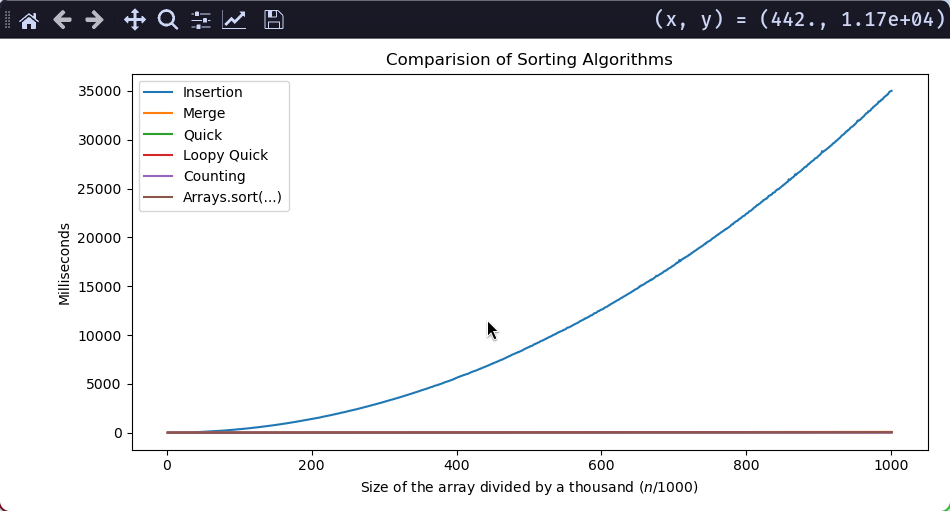
\includegraphics[width=\linewidth]{plotbig.png}
\end{figure}

\begin{figure}
  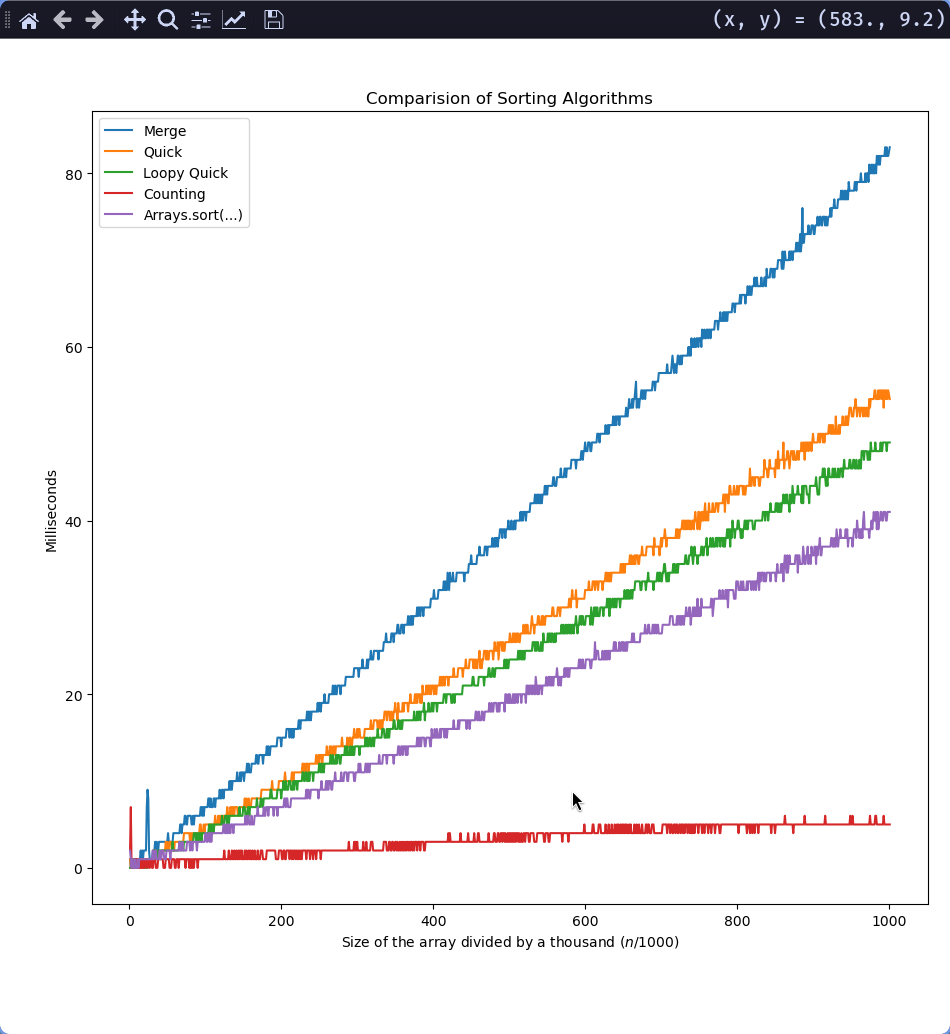
\includegraphics[width=\linewidth]{Screenshot_19-Sep_10-03-32_matplotlib.png}
\end{figure}


\section*{Submission Instructions}

\begin{enumerate}
  \item Turn in a PDF containing any plots and answers from the homework.
  \item Also turn in your \texttt{Sorter.java}. Note that since you may
        not change anything in either \texttt{Experiment.java} or
        \texttt{GodricsHat.java}, there is no need to turn those in.
\end{enumerate}

\end{document}
